
\begin{center}
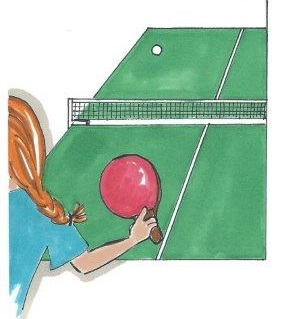
\includegraphics[width=0.4\textwidth]{content/3/chapter7/images/1.png}\\
Cippi在打乒乓球
\end{center}

\begin{tcolorbox}[breakable,enhanced jigsaw,colback=blue!5!white,colframe=blue!75!black,title={具体设备的性能参考}]
对性能数据应该持保留态度,我对Linux和Windows上每种算法变体的性能数字不感兴趣。我更感兴趣的是一种直觉,哪些算法可能有效或无效。我并不是在比较我的Linux桌面和Windows笔记本电脑上的绝对数字,但我想知道某些算法在Linux或Windows上可以运行得更好。
\end{tcolorbox}

当要多次同步线程时,可以使用条件变量、std::atomic\_flag、std::atomic<bool>或信号量。本节中,我要回答的问题是:哪种方式最快?

为了得到类似的数字,我实现了一个乒乓球游戏。一个线程执行ping函数(或简称ping线程),另一个线程执行pong函数(或简称pong线程)。ping线程等待pong线程通知,并将通知发送回pong线程,100万次“打击”后比赛结束。我将每款游戏执行5次,以获得可比较的性能数据。

\begin{tcolorbox}[breakable,enhanced jigsaw,colback=blue!5!white,colframe=blue!75!black,title={关于数字}]
我在2020年底用全新的Visual Studio编译器19.28进行了性能测试,该编译器支持与原子(std::atomic\_flag和std::atomic)和信号量的同步。此外,我用最大优化(/Ox)编译了这些示例。性能值只能大致说明同步线程的各种方法的相对性能。若想在平台上获得准确的数字,必须重复进行测试。
\end{tcolorbox}

先与C++11进行比较。

\subsubsubsection{7.1.1\hspace{0.2cm}条件变量}

\begin{lstlisting}[style=styleCXX]
// pingPongConditionVariable.cpp

#include <condition_variable>
#include <iostream>
#include <atomic>
#include <thread>

bool dataReady{false};

std::mutex mutex_;
std::condition_variable condVar1;
std::condition_variable condVar2;

std::atomic<int> counter{};
constexpr int countlimit = 1'000'000;

void ping() {

	while(counter <= countlimit) {
		{
			std::unique_lock<std::mutex> lck(mutex_);
			condVar1.wait(lck, []{return dataReady == false;});
			dataReady = true;
		}
		++counter;
		condVar2.notify_one();
	}
}

void pong() {

	while(counter < countlimit) {
		{
			std::unique_lock<std::mutex> lck(mutex_);
			condVar2.wait(lck, []{return dataReady == true;});
			dataReady = false;
		}
		condVar1.notify_one();
	}

}

int main(){

	auto start = std::chrono::system_clock::now();
	
	std::thread t1(ping);
	std::thread t2(pong);
	
	t1.join();
	t2.join();
	
	std::chrono::duration<double> dur = std::chrono::system_clock::now() - start;
	std::cout << "Duration: " << dur.count() << " seconds" << '\n';
}
\end{lstlisting}

程序中使用了两个条件变量:condVar1和condVar2。ping线程等待condVar1的通知,并将其通知与condVar2一起发送,dataReady可以防止伪和未唤醒。当计数器达到计数限时,乒乓球比赛结束。调用notify\_one(第26行和第38行)和计数器是线程安全的,因此不在临界区内。

下面就是数据。

\begin{center}
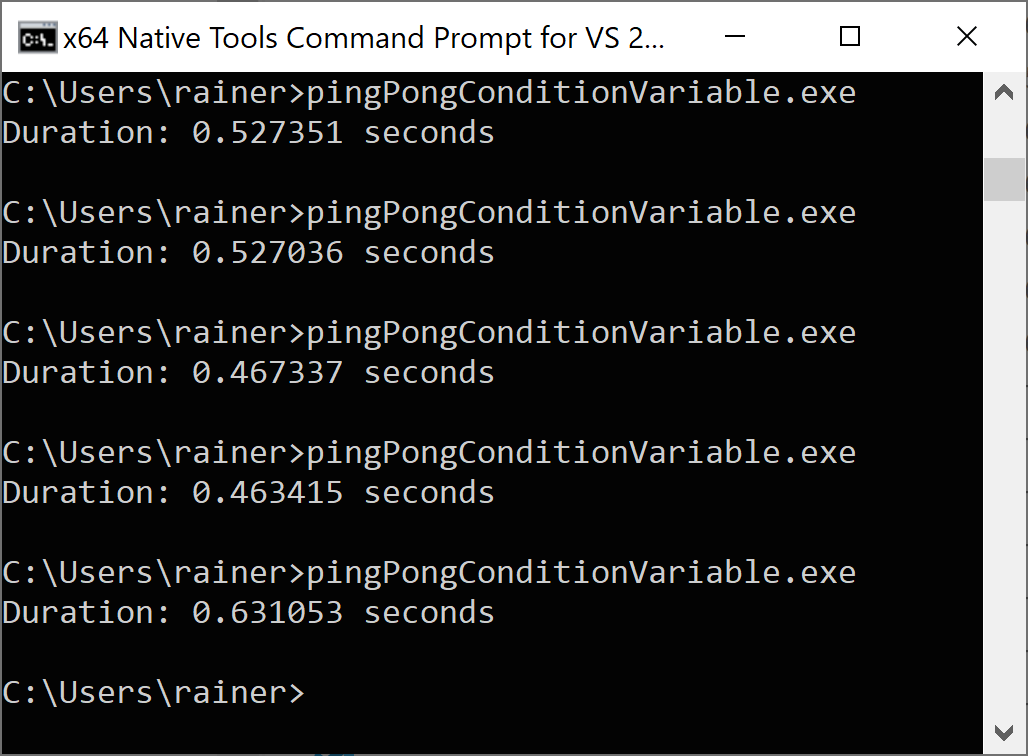
\includegraphics[width=0.6\textwidth]{content/3/chapter7/images/2.png}\\
\end{center}

平均执行时间为0.52秒。

C++20中,将这个工作流移植到std::atomic\_flag很简单。

\subsubsubsection{7.1.2\hspace{0.2cm}std::atomic\_flag}

下面是使用两个原子标志和一个原子标志的相同工作流。

\hspace*{\fill} \\ %插入空行
\noindent
\textbf{7.1.2.1\hspace{0.2cm}两个原子标志}

下面的程序中,我将条件变量的等待替换为对原子标志的等待,并将条件变量的通知替换为原子标志设置后的通知。

\begin{lstlisting}[style=styleCXX]
// pingPongAtomicFlags.cpp

#include <iostream>
#include <atomic>
#include <thread>

std::atomic_flag condAtomicFlag1{};
std::atomic_flag condAtomicFlag2{};

std::atomic<int> counter{};
constexpr int countlimit = 1'000'000;
void ping() {
	while(counter <= countlimit) {
		condAtomicFlag1.wait(false);
		condAtomicFlag1.clear();
		
		++counter;
		
		condAtomicFlag2.test_and_set();
		condAtomicFlag2.notify_one();
	}
}

void pong() {
	while(counter < countlimit) {
		condAtomicFlag2.wait(false);
		condAtomicFlag2.clear();
		
		condAtomicFlag1.test_and_set();
		condAtomicFlag1.notify_one();
	}
}

int main() {

	auto start = std::chrono::system_clock::now();
	
	condAtomicFlag1.test_and_set();
	std::thread t1(ping);
	std::thread t2(pong);
	
	t1.join();
	t2.join();
	
	std::chrono::duration<double> dur = std::chrono::system_clock::now() - start;
	std::cout << "Duration: " << dur.count() << " seconds" << '\n';

}
\end{lstlisting}

若原子标志的值为false,condAtomicFlag1.wait(false)(第15行)将阻塞;若condAtomicFlag1的值为true,则返回。布尔值作为一种谓词,因此设置为false(第15行)。将通知(第21行)发送到pong线程之前,condAtomicFlag1设置为true(第20行)。condAtomicFlag1(第39行)的初始设置为true,开始游戏。

因为使用了std::atomic\_flag,游戏结束得更快了。

\begin{center}
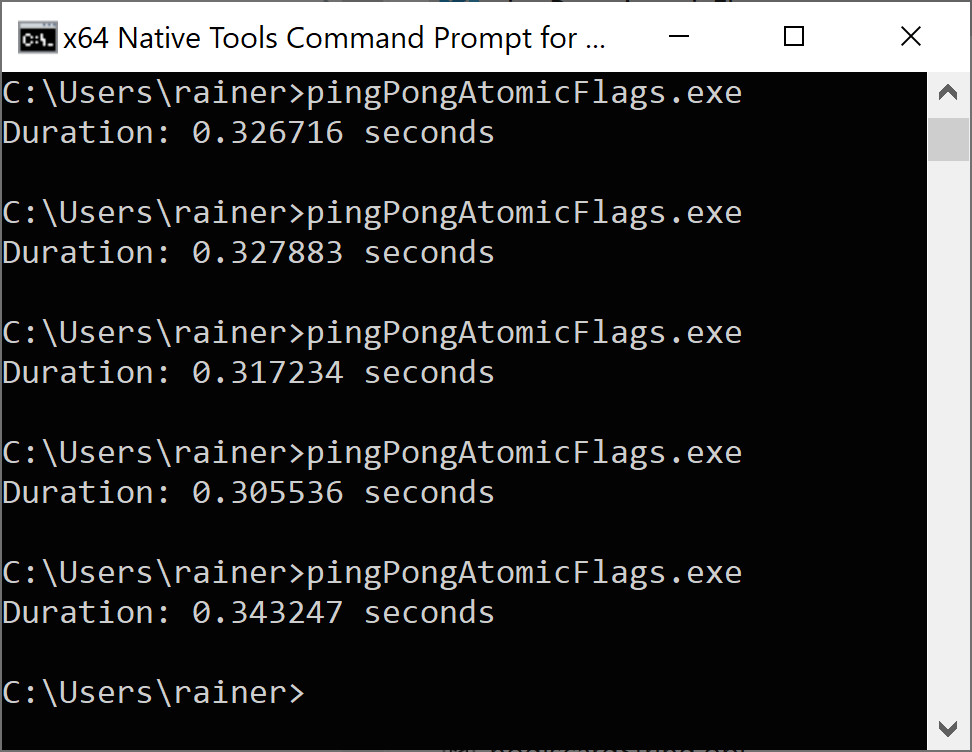
\includegraphics[width=0.6\textwidth]{content/3/chapter7/images/3.png}\\
\end{center}

一场游戏平均需要0.32秒。

当分析程序时,可能会觉得一个原子标志对于这个工作流来说足够了。

\hspace*{\fill} \\ %插入空行
\noindent
\textbf{7.1.2.2\hspace{0.2cm}一个原子标志}

使用一个原子标志使工作流更容易理解。

\begin{lstlisting}[style=styleCXX]
// pingPongAtomicFlag.cpp

#include <iostream>
#include <atomic>
#include <thread>

std::atomic_flag condAtomicFlag{};

std::atomic<int> counter{};
constexpr int countlimit = 1'000'000;

void ping() {
	while(counter <= countlimit) {
		condAtomicFlag.wait(true);
		condAtomicFlag.test_and_set();
		
		++counter;
		
		condAtomicFlag.notify_one();
	}
}

void pong() {
	while(counter < countlimit) {
		condAtomicFlag.wait(false);
		condAtomicFlag.clear();
		condAtomicFlag.notify_one();
	}
}

int main() {

	auto start = std::chrono::system_clock::now();
	
	condAtomicFlag.test_and_set();
	std::thread t1(ping);
	std::thread t2(pong);
	
	t1.join();
	t2.join();
	
	std::chrono::duration<double> dur = std::chrono::system_clock::now() - start;
	std::cout << "Duration: " << dur.count() << " seconds" << '\n';

}
\end{lstlisting}

ping线程阻塞在true上,而pong线程阻塞在false上。从性能的角度来看,使用一个或两个原子标志没有区别。

\begin{center}
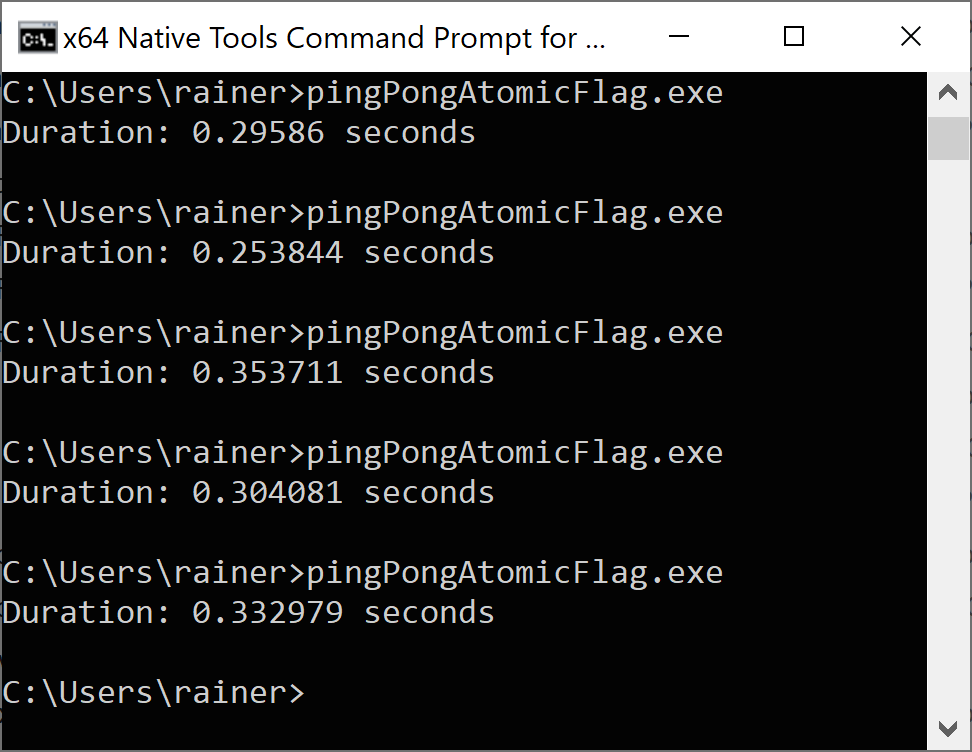
\includegraphics[width=0.6\textwidth]{content/3/chapter7/images/4.png}\\
\end{center}

执行的平均时间为0.31秒。

这个例子中,我使用std::atomic\_flag作为原子布尔值。让我们用std::atomic<bool>再试一次。

\subsubsubsection{7.1.3\hspace{0.2cm}std::atomic<bool>}

下面的C++20基于std::atomic的实现。

\begin{lstlisting}[style=styleCXX]
// pingPongAtomicBool.cpp

#include <iostream>
#include <atomic>
#include <thread>

std::atomic<bool> atomicBool{};

std::atomic<int> counter{};
constexpr int countlimit = 1'000'000;

void ping() {
	while(counter <= countlimit) {
		atomicBool.wait(true);
		atomicBool.store(true);
		
		++counter;
		
		atomicBool.notify_one();
	}
}

void pong() {
	while(counter < countlimit) {
		atomicBool.wait(false);
		atomicBool.store(false);
		atomicBool.notify_one();
	}
}

int main() {

	std::cout << std::boolalpha << '\n';
	
	std::cout << "atomicBool.is_lock_free(): "
	<< atomicBool.is_lock_free() << '\n';
	
	std::cout << '\n';
	
	auto start = std::chrono::system_clock::now();
	
	atomicBool.store(true);
	std::thread t1(ping);
	std::thread t2(pong);
	
	t1.join();
	t2.join();
	
	std::chrono::duration<double> dur = std::chrono::system_clock::now() - start;
	std::cout << "Duration: " << dur.count() << " seconds" << '\n';

}
\end{lstlisting}

std::atomic<bool>可以在内部使用锁,例如:互斥锁。Windows在运行时是无锁的。

\begin{center}
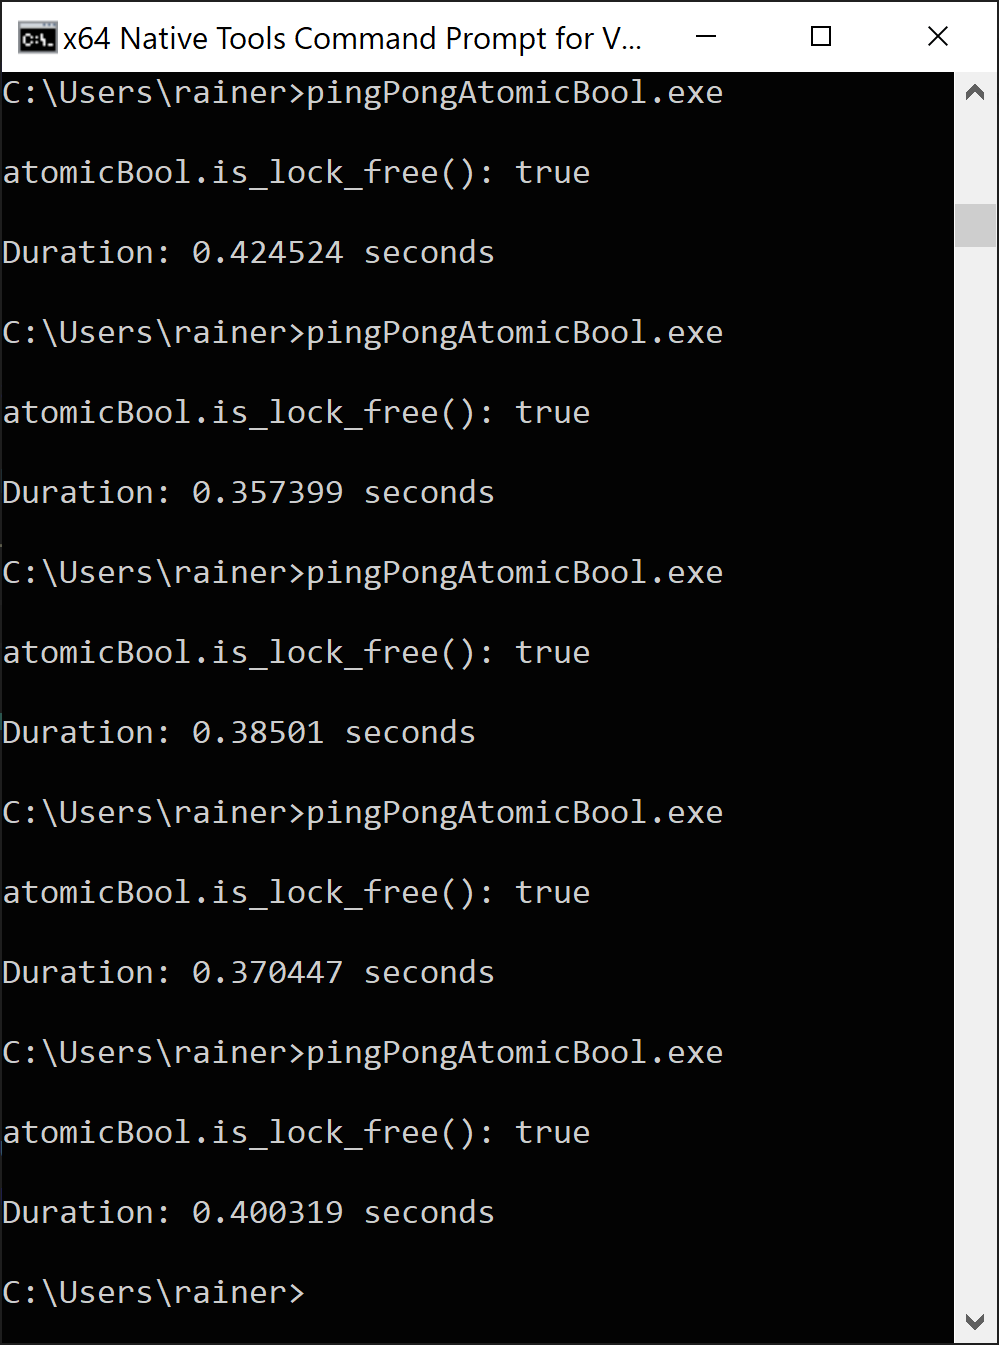
\includegraphics[width=0.6\textwidth]{content/3/chapter7/images/5.png}\\
\end{center}

平均执行时间为0.38秒。

从可读性的角度来看,这个基于std::atomic的实现很容易理解。这个观察结果也适用于基于信号量实现的乒乓游戏。

\subsubsubsection{7.1.4\hspace{0.2cm}信号量}

信号量比条件变量更快,来看看这是不是真的。

\begin{lstlisting}[style=styleCXX]
// pingPongSemaphore.cpp

#include <iostream>
#include <semaphore>
#include <thread>

std::counting_semaphore<1> signal2Ping(0);
std::counting_semaphore<1> signal2Pong(0);

std::atomic<int> counter{};
constexpr int countlimit = 1'000'000;

void ping() {
	while(counter <= countlimit) {
		signal2Ping.acquire();
		++counter;
		signal2Pong.release();
	}
}

void pong() {
	while(counter < countlimit) {
		signal2Pong.acquire();
		signal2Ping.release();
	}
}

int main() {

	auto start = std::chrono::system_clock::now();
	
	signal2Ping.release();
	std::thread t1(ping);
	std::thread t2(pong);
	
	t1.join();
	t2.join();
	
	std::chrono::duration<double> dur = std::chrono::system_clock::now() - start;
	std::cout << "Duration: " << dur.count() << " seconds" << '\n';

}
\end{lstlisting}

pingpongsemapore.cpp使用了两个信号量:signal2Ping和signal2Pong(第7行和第8行)。这两个信号量都可以有0或1,并都初始化为0。当信号量signal2Ping的值为0时,signal2Ping.release()(第24和32行)将该值设置为1,因此这是一个通知。signal2Ping.acquire()(第15行)进行阻塞,直到值变为1。同样的方式,也适用于第二个信号量signal2Pong。

\begin{center}
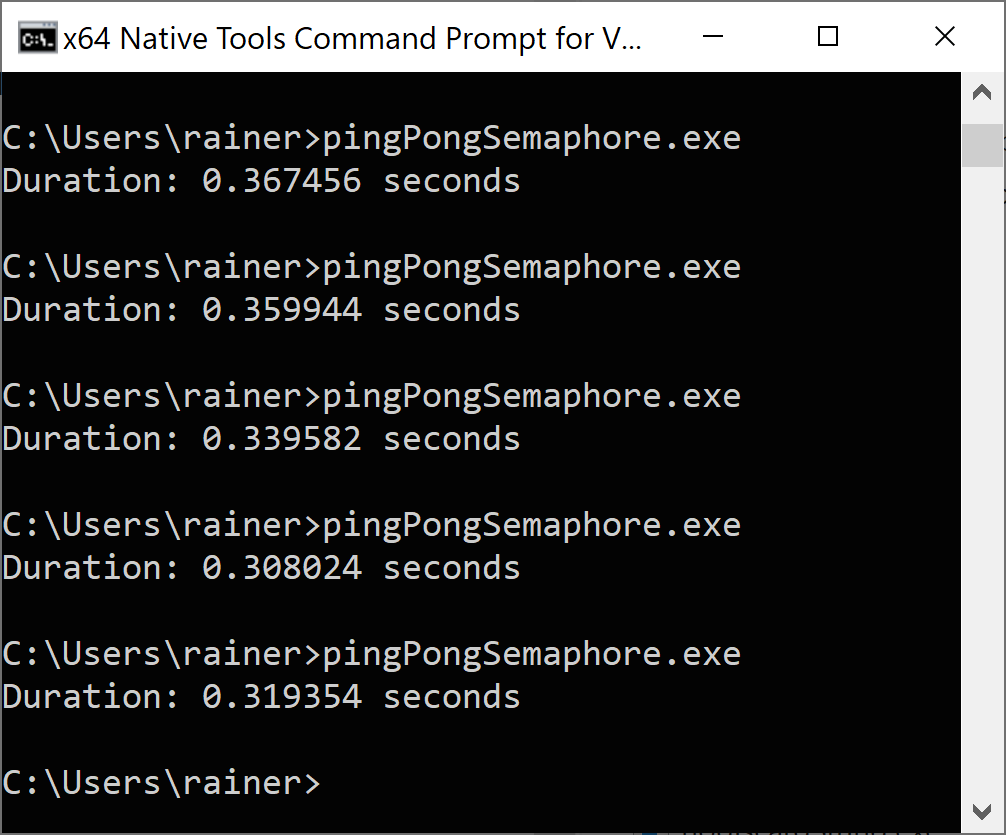
\includegraphics[width=0.6\textwidth]{content/3/chapter7/images/6.png}\\
\end{center}

平均执行时间为0.33秒。

\subsubsubsection{7.1.5\hspace{0.2cm}所有的数据}

如预期的那样,条件变量是最慢的方式,原子标记是同步线程的最快方式。std::atomic<bool>的性能介于两者之间。std::atomic<bool>有一个缺点,是唯一无锁的原子数据类型。信号量给我的印象最深,因为它几乎与原子标志一样快。

\begin{table}[H]
\centering
\begin{tabular}{llllll}
&
\textbf{\begin{tabular}[c]{@{}l@{}}条件\\ 变量\end{tabular}} &
\textbf{\begin{tabular}[c]{@{}l@{}}两个原子\\ 标志\end{tabular}} &
\textbf{\begin{tabular}[c]{@{}l@{}}一个原子\\ 标志\end{tabular}} &
\textbf{\begin{tabular}[c]{@{}l@{}}原子\\ 布尔\end{tabular}} &
\textbf{信号量} \\ \hline
\textbf{\begin{tabular}[c]{@{}l@{}}执行 \\ 时间(秒)\end{tabular}} &
0.52 &
0.32 &
0.31 &
0.38 &
0.33
\end{tabular}
\end{table}

\newpage










